\documentclass{beamer}
\usepackage{amsfonts,amsmath,oldgerm}
\usetheme{sintef}
\usepackage{xeCJK}
\newcommand{\testcolor}[1]{\colorbox{#1}{\textcolor{#1}{test}}~\texttt{#1}}
\usefonttheme[onlymath]{serif}
\titlebackground*{figures/background}
\newcommand{\hrefcol}[2]{\textcolor{cyan}{\href{#1}{#2}}}

% Page 1

\title{智慧幕墙:系统架构与服务器运维}
\subtitle{Intelligent Curtain Wall: System Architecture and Server Operations and Maintenance}
\course{计算机科学与技术学院}
\author{林继申、刘淑仪、中谷天音}
\date{2024年11月13日}

\begin{document}
\maketitle

% Page 2

\section{项目目标}

% Page 3

\subsection{项目存在问题}

\begin{frame}[fragile]{项目存在问题}
\framesubtitle{Project Issues}
\begin{columns}
\begin{column}{0.7\textwidth}
\begin{enumerate}
\item 环境依赖问题
\begin{itemize}
\item 各开发环境不一致,导致代码在不同环境下表现不一。
\item 开发人员常遇到“本地测试没问题,但在他人电脑或部署环境中出错”的问题。
\end{itemize}
\item 开发效率低下
\begin{itemize}
\item 缺乏规范的Git操作流程,代码冲突频繁。
\item 没有使用分支、Pull Request等最佳实践,导致代码管理混乱。
\end{itemize}
\item 手动部署耗时且易出错
\begin{itemize}
\item 部署过程依赖人工操作,需要手动拉取代码、配置环境并部署。
\item 部署流程繁琐且容易出错,部署滞后,开发完成的代码无法及时上线。
\end{itemize}
\end{enumerate}
\end{column}
\begin{column}{0.3\textwidth}
\begin{block}{项目必要性}
\begin{itemize}
\item 解决环境依赖问题,提升开发稳定性
\item 提升团队协作效率,减少代码冲突
\item 部署自动化,缩短交付周期
\item 支持快速迭代与反馈,及时响应需求变化
\end{itemize}
\end{block}
\end{column}
\end{columns}
\end{frame}

% Page 4

\subsection{用户需求与系统需求}

\begin{frame}[fragile]{用户需求与系统需求}
\framesubtitle{User Requirements and System Requirements}
\begin{columns}
\begin{column}{0.7\textwidth}
用户需求:
\begin{enumerate}
\item \footnotesize 环境一致性
\begin{itemize}
\item \footnotesize 用户痛点:环境不一致导致的运行错误。
\item \footnotesize 示例问题:本地测试通过,但在其他环境中出现问题。
\end{itemize}
\item \footnotesize 高效协作
\begin{itemize}
\item \footnotesize 用户痛点:开发过程中频繁发生代码冲突,影响进度。
\item \footnotesize 示例问题:缺乏规范化的Git操作流程和分支管理。
\end{itemize}
\item \footnotesize 快速部署与更新
\begin{itemize}
\item \footnotesize 用户痛点:手动部署耗时且易出错,影响功能上线时间。
\item \footnotesize 需求期望:希望通过自动化部署实现快速上线。
\end{itemize}
\item \footnotesize 快速迭代与反馈
\begin{itemize}
\item \footnotesize 用户痛点:难以及时响应需求的变化,更新上线周期过长。
\item \footnotesize 需求期望:希望通过敏捷方法快速迭代。
\end{itemize}
\end{enumerate}
\end{column}
\begin{column}{0.3\textwidth}
系统需求:
\begin{enumerate}
\item \footnotesize 技术需求
\begin{itemize}
\item \footnotesize 一致的环境配置
\item \footnotesize 自动化部署
\end{itemize}
\item \footnotesize 代码管理需求
\begin{itemize}
\item \footnotesize 高效的版本控制
\end{itemize}
\item \footnotesize 系统集成需求
\begin{itemize}
\item \footnotesize 模块化系统架构
\end{itemize}
\item \footnotesize 性能需求
\begin{itemize}
\item \footnotesize 快速部署与更新
\end{itemize}
\item \footnotesize 团队协作需求
\begin{itemize}
\item \footnotesize 敏捷开发支持
\end{itemize}
\end{enumerate}
\end{column}
\end{columns}
\end{frame}

% Page 5

\subsection{项目核心目标}

\begin{frame}[fragile]{项目核心目标}
\framesubtitle{Project Core Objectives}
\begin{enumerate}
\item 解决环境依赖问题
\begin{itemize}
\item 引入Docker技术,确保开发、测试、生产环境一致。
\item 使用Docker Compose进行统一环境配置,消除“环境不一致”导致的问题。
\end{itemize}
\item 提升开发效率
\begin{itemize}
\item 通过Git的Submodule机制和最佳实践,实现代码独立管理与高效集成。
\item 使用分支管理、PR流程等,降低代码冲突,提高协作效率。
\end{itemize}
\item 实现自动化部署
\begin{itemize}
\item 引入CI/CD流水线,自动化构建、测试、部署流程。
\item 服务器定时拉取最新镜像并自动部署,确保开发完成的功能能快速上线。
\end{itemize}
\item 加速项目迭代
\begin{itemize}
\item 缩短从开发到上线的周期,快速验证和反馈。
\item 通过高效的迭代流程,保证产品质量和交付速度。
\end{itemize}
\end{enumerate}
\end{frame}

% Page 6

\section{项目范围与约束}

% Page 7

\subsection{项目范围}

\begin{frame}[fragile]{项目范围}
\framesubtitle{Project Scope}
\begin{columns}
\begin{column}{0.85\textwidth}
\begin{enumerate}
\item 技术栈范围
\begin{itemize}
\item 各子系统的开发均基于Docker技术,提供一致的开发环境。
\item 使用Git的Submodule机制,实现代码的独立管理与集成。
\item 集成CI/CD工具(GitHub Actions)用于自动化构建与部署。
\end{itemize}
\item 团队管理
\begin{itemize}
\item 36人的团队分为10组,各自负责不同子系统的开发。
\item 每组拥有独立的Git仓库,并遵循最佳git实践(分支管理、PR流程等)。
\end{itemize}
\item 子系统与集成
\begin{itemize}
\item 项目包含11个子系统,每个子系统由不同小组独立开发。
\item 使用Docker Compose进行11个子系统的集成与统一部署。
\end{itemize}
\item 部署与生产环境
\begin{itemize}
\item 部署环境采用Docker Compose,确保生产环境与开发环境一致。
\item 服务器自动定时从Docker Hub拉取最新镜像,更新生产环境。
\end{itemize}
\end{enumerate}
\end{column}
\begin{column}{0.15\textwidth}

\includegraphics[width=\textwidth]
{figures/docker}

\includegraphics[width=\textwidth]
{figures/docker_compose}

\includegraphics[width=\textwidth]
{figures/git}

\includegraphics[width=\textwidth]
{figures/github_actions}
\end{column}
\end{columns}
\end{frame}

% Page 8

\subsection{项目约束}

\begin{frame}[fragile]{项目约束}
\framesubtitle{Project Constraints}
\begin{enumerate}
\item 技术约束
\begin{itemize}
\item 所有开发必须基于Docker进行,确保环境一致性。
\item 代码管理必须严格遵循Git最佳实践,包括分支策略、PR审核等。
\end{itemize}
\item 时间约束
\begin{itemize}
\item 每半小时服务器自动拉取最新镜像进行部署。
\item 项目整体需在既定时间内完成,并且各小组的子系统需要定期交付版本。
\end{itemize}
\item 资源约束
\begin{itemize}
\item CI/CD流水线和Docker Compose部署需要占用服务器资源,需合理配置服务器。
\item 团队内的沟通与协作需要配备相应的工具(如微信、飞书、GitHub等)以提高效率。
\end{itemize}
\item 人员约束
\begin{itemize}
\item 每组需要保证独立性,但必须定期将成果集成到主仓库。
\item 需确保团队成员熟悉Git、Docker、CI/CD工具等技术,以避免因技术门槛导致的延误。
\end{itemize}
\end{enumerate}
\end{frame}

% Page 9

\section{用户参与 / 过程模型}

% Page 10

\subsection{用户参与过程(系统开发流程)}

\begin{frame}[fragile]{用户参与过程(系统开发流程)}
\framesubtitle{User Involvement Process (System Development Lifecycle)}
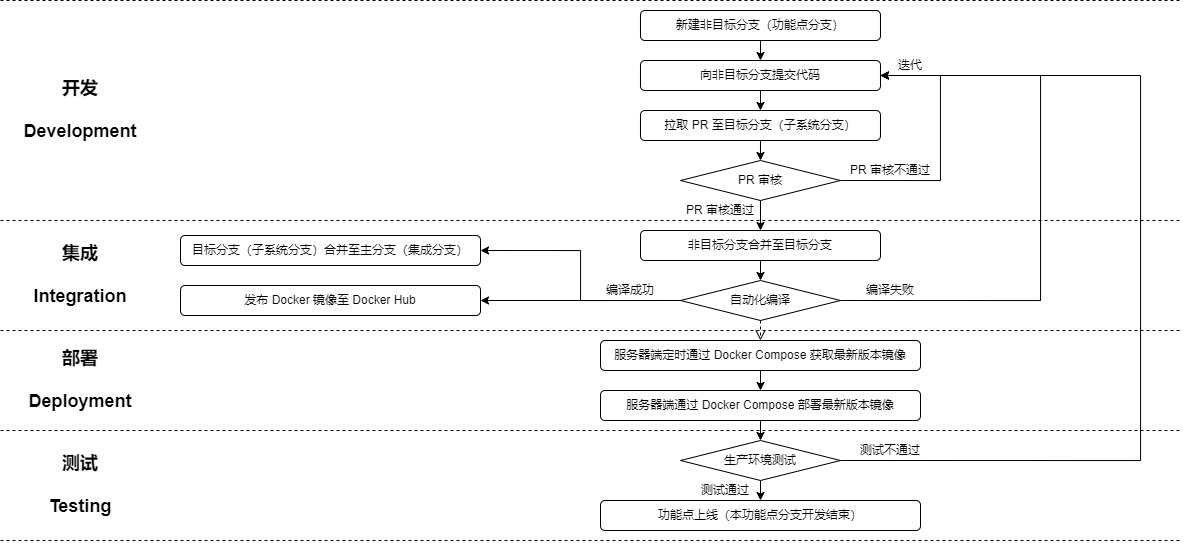
\includegraphics[width=\textwidth]
{figures/system_development_flowchart}
\end{frame}

% Page 11

\subsection{敏捷Scrum框架}

\begin{chapter}[figures/background_negative]{}{敏捷Scrum框架}
\framesubtitle{Agile Scrum Framework}
\begin{itemize}
\item 敏捷Scrum优势
\item Scrum开发流程
\item Scrum项目进展
\end{itemize}
\end{chapter}

% Page 12

\begin{frame}[fragile]{敏捷Scrum优势}
\framesubtitle{Advantages of Agile Scrum}
\begin{columns}
\begin{column}{0.55\textwidth}
Scrum是一种敏捷开发方法论,专注于通过小团队合作以及快速频繁的迭代来管理和完成复杂的软件和非软件项目。Scrum的优势如下:
\begin{itemize}
\item \footnotesize 灵活性与适应性:Scrum允许在项目开发过程中快速适应变化,这对于需求不断变化的项目环境尤为重要。
\item \footnotesize 增强透明度:通过日常站会和冲刺回顾,项目进度和障碍对所有团队成员都是透明的,增强了团队的沟通和协作。
\item \footnotesize 持续改进:每次冲刺结束时的回顾会帮助团队评估其效率和工作方式,不断寻找改进的机会。
\item \footnotesize 快速迭代:短周期的工作冲刺使团队能够快速交付产品特性,及时响应市场和客户的反馈。
\end{itemize}
\end{column}
\begin{column}{0.45\textwidth}

\includegraphics[width=\textwidth]
{figures/scrum}
\end{column}
\end{columns}
\end{frame}

% Page 13

\begin{frame}[fragile]{Scrum开发流程}
\framesubtitle{Scrum Development Process}
\begin{columns}
\begin{column}{0.5\textwidth}
\footnotesize 考虑到本项目涉及多个子系统和一个由36人组成的较大团队,使用Scrum框架可以有效地管理多元化的需求和快速变化的开发环境。
\begin{block}{Scrum实施步骤}
\footnotesize Sprint计划会议→每日站会→持续集成与部署→Sprint评审会→Sprint回顾会
\end{block}
\begin{block}{特定优化措施}
\begin{enumerate}
\item \footnotesize 使用Docker和CI/CD可以极大地支持Scrum的快速迭代特性,通过自动化测试和部署,缩短开发周期,减少人工错误。
\item \footnotesize 通过Git的Submodule机制,各子系统独立但集成,使得Scrum团队能够更有效地协作,同时保持代码的整洁和管理的可控性。
\end{enumerate}
\end{block}
\end{column}
\begin{column}{0.5\textwidth}
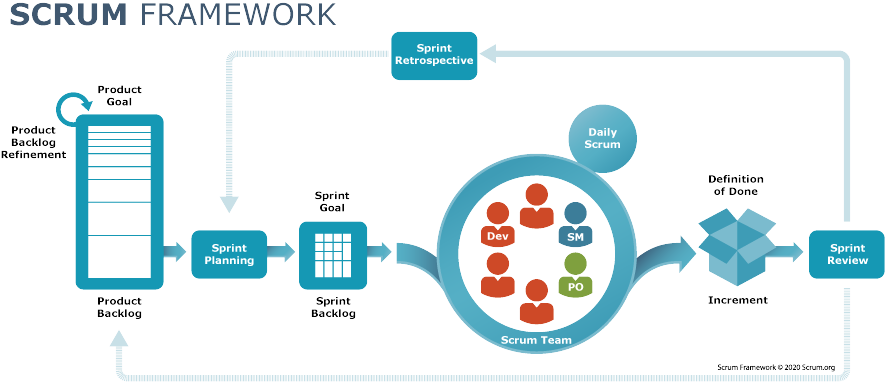
\includegraphics[width=\textwidth]
{figures/scrum_framework}
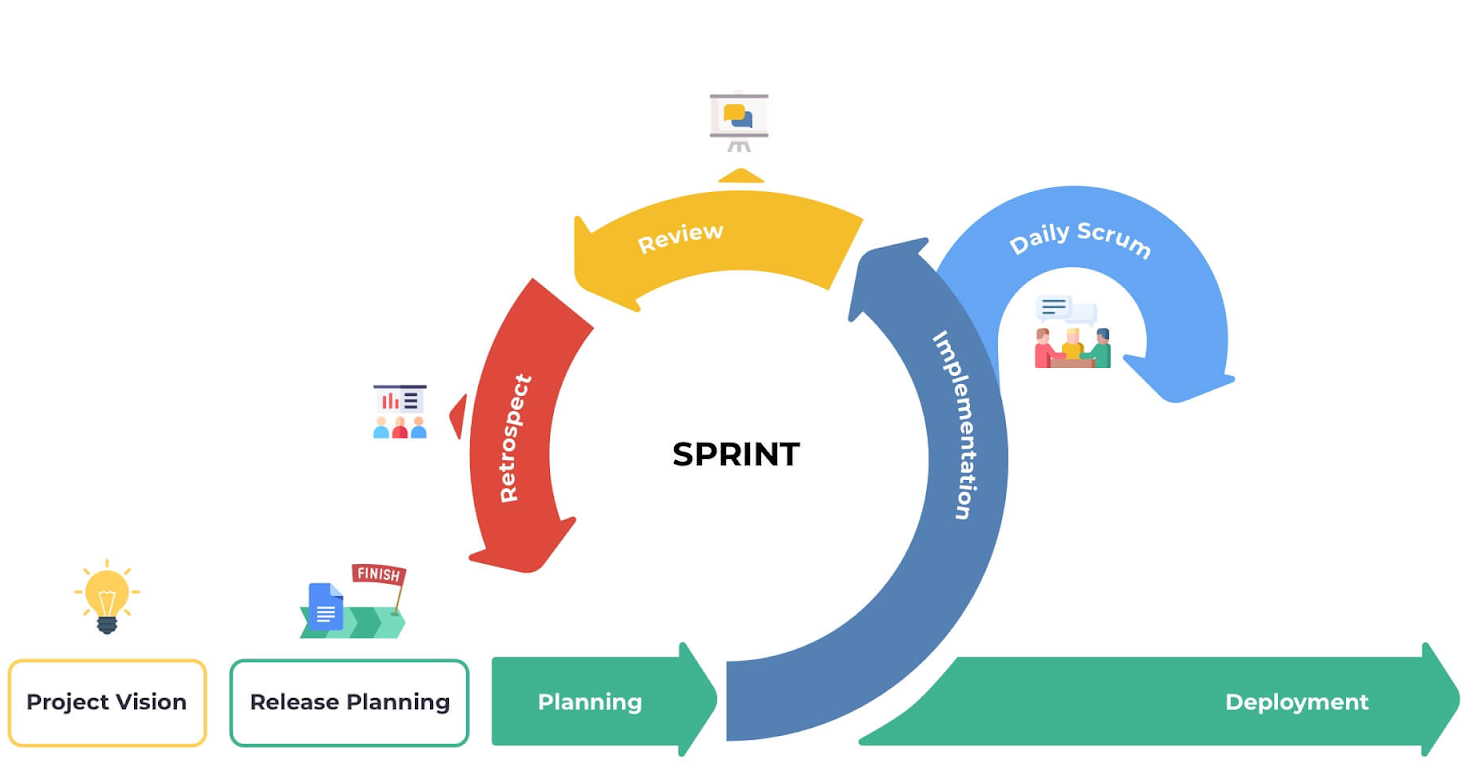
\includegraphics[width=\textwidth]
{figures/scrum_sprint}
\end{column}
\end{columns}
\end{frame}

% Page 14

\begin{frame}[fragile]{Scrum项目进展}
\framesubtitle{Scrum Project Progress}
\begin{columns}
\begin{column}{0.3\textwidth}
\begin{colorblock}[white]{sintefyellow}{已完成}
\footnotesize 环境依赖问题解决:使用Docker和Docker Compose,确保开发、测试、生产环境一致。

\vspace{\baselineskip}

\footnotesize 代码管理优化:通过Git Submodule机制,建立各子系统独立的仓库管理,同时引入分支管理、Pull Request等最佳实践。

\vspace{\baselineskip}

\footnotesize 自动化部署实现:配置CI/CD流水线,代码提交后自动触发构建、测试和部署。服务器定时更新镜像并重新部署。
\end{colorblock}
\end{column}
\begin{column}{0.3\textwidth}
\begin{colorblock}[white]{sintefgreen}{进展中}
\footnotesize 快速迭代流程建立:每周进行Sprint规划、迭代开发和回顾,不断优化开发流程。

\vspace{\baselineskip}

\footnotesize 收集小组反馈,完善系统架构:持续收集各个小组的意见和建议,针对系统架构和开发流程进行优化,以适应项目的复杂性和团队协作需求。

\vspace{5\baselineskip}
\end{colorblock}
\end{column}
\begin{column}{0.3\textwidth}
\begin{colorblock}[white]{maincolor}{待完成}
\footnotesize 项目中的图片数据集通过阿里云OSS对象存储进行管理和维护,确保数据存储高效、安全、可扩展。各小组可以便捷地访问和更新数据集,实现开发与测试资源的统一管理。

\vspace{8\baselineskip}
\end{colorblock}
\end{column}
\end{columns}
\end{frame}

% Page 15

\section{交流问题}

% Page 16

\begin{frame}[fragile]{交流问题}
\framesubtitle{Communication Issues}
\begin{itemize}
\item 确保团队成员之间的信息流通顺畅,尤其是在敏捷Scrum框架下,日常站会和Sprint回顾要确保及时共享进展与问题。
\item 建立清晰的沟通渠道,如微信群或飞书等工具,避免信息滞后或误解。
\item 处理反馈时要注重倾听和反馈的及时性,避免因沟通不畅导致项目进度或质量的影响。
\item 随着项目的推进,技术架构、开发流程、CI/CD配置等方面的文档及时更新,确保每个团队成员都能访问到最新的工作信息和系统架构设计。这对于跨团队合作尤为重要。
\begin{itemize}
\item 《后端技术选型——Docker Compose技术栈》
\item 《Git版本控制系统基本操作指南》
\item 《智慧幕墙项目后端应用程序集成Git开发规范与流程》
\end{itemize}
\end{itemize}
\end{frame}

% Page 17

\section{获取方法}

% Page 18

\begin{frame}[fragile]{获取方法}
\framesubtitle{Acquisition Method}
\begin{columns}
\begin{column}{0.45\textwidth}
项目的获取方法如下:
\begin{enumerate}
\item 科研项目需求
\begin{itemize}
\item 项目来源于科研任务或学术研究的需求。
\end{itemize}
\item 开发团队内部反馈
\begin{itemize}
\item 项目由开发团队在日常工作中发现的问题或改进点推动立项。
\end{itemize}
\end{enumerate}
根据项目需求来源,可以灵活调整项目目标和实施策略,确保科研和开发目标都能高效实现。
\end{column}
\begin{column}{0.45\textwidth}

\includegraphics[width=\textwidth]
{figures/acquisition_method}
\end{column}
\end{columns}
\end{frame}

% Page 19

\backmatter
\end{document}